% 2007 江苏 Q19 图
% 抛物线 y=x^2; C(0,2) 在 y 轴正方向; 直线 AB: y=x+2 交抛物线于 A(-1,1), B(2,4);
% 垂直 x 轴的直线 x=1/2 交 AB 于中点 P(1/2,5/2), 交 l:y=-2 于 Q(1/2,-2); QA 为 A 处切线 y=-2x-1。
\usetikzlibrary{arrows.meta,calc}
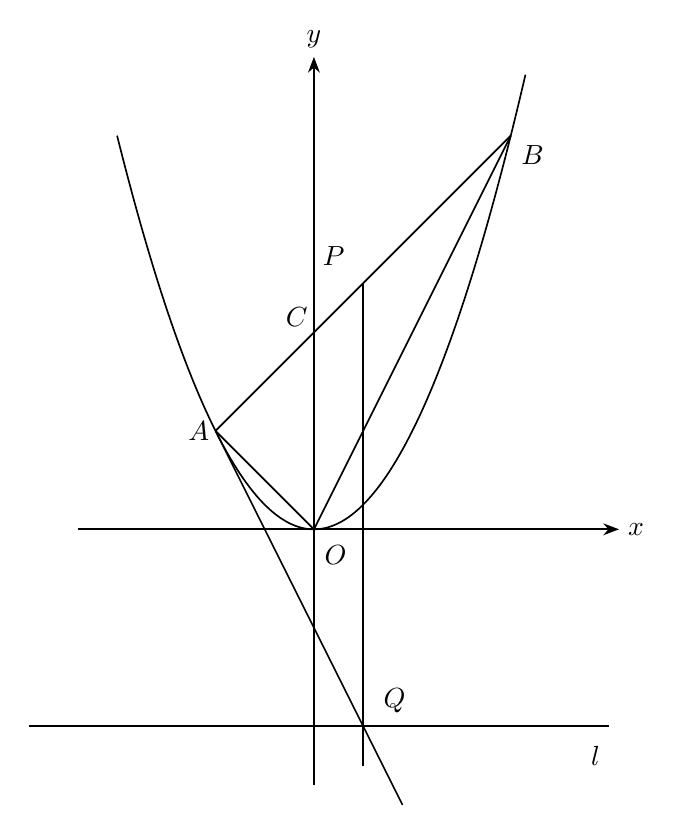
\begin{tikzpicture}[x=1.25cm,y=1.25cm,line width=.6pt,font=\normalsize,>=Stealth,
  lbl/.style={inner sep=1pt}]
\coordinate (O) at (0,0);
\coordinate (A) at (-1,1);
\coordinate (B) at (2,4);
\coordinate (C) at (0,2);
\coordinate (P) at (0.5,2.5);
\coordinate (Q) at (0.5,-2);
% 抛物线 y=x^2
\draw[domain=-2.0:2.15,samples=121] plot (\x,{\x*\x});
% 直线 AB: y=x+2
\draw (A)--(B);
% OA, OB
\draw (O)--(A);
\draw (O)--(B);
% A 处切线 QA: y=-2x-1, 越过 Q 延长
\draw (-1,1)--(0.9,-2.8);
% 垂直于 x 轴的直线 x=1/2, 过 P, Q
\draw (0.5,2.5)--(0.5,-2.4);
% 准线 l: y=-2
\draw (-2.9,-2)--(3.0,-2);
\draw[->] (-2.4,0)--(3.1,0) node[lbl,right,xshift=2pt] {$x$};
\draw[->] (0,-2.6)--(0,4.8) node[lbl,above,yshift=2pt] {$y$};
\node[lbl] at (0.22,-0.26) {$O$};
\node[anchor=south east,inner sep=0pt,xshift=-2pt,yshift=2pt] at (C) {$C$};
\node[anchor=east,inner sep=0pt,xshift=-2pt] at (A) {$A$};
\node[lbl] at (2.22,3.80) {$B$};
\node[lbl] at (0.20,2.78) {$P$};
\node[lbl] at (0.82,-1.74) {$Q$};
\node[lbl] at (2.86,-2.30) {$l$};
\end{tikzpicture}
